\documentclass[10pt, a4paper,german]{scrartcl}
%\oddsidemargin-0.5cm
%\textwidth17cm
%\addtolength{\voffset}{1cm}
%\topskip-1cm
%\topmargin-1cm
%\usepackage[headlines=2.1]{typearea}
%\headheight=5cm
\usepackage{babel}
\usepackage{tabularx}
\usepackage{graphicx}
\usepackage{eurosym}
\usepackage{booktabs}
\usepackage{fontspec}
\usepackage{listings}
\usepackage{xcolor}
\usepackage[iso]{isodate}
%
\usepackage{amsmath}
%\usepackage{amsops} % DeclarMathOperator
%
\usepackage[bookmarks,colorlinks,linkcolor=blue]{hyperref}
%\usepackage{sbericht}
\usepackage{scrlayer-scrpage}

  \newcommand*{\name}[1]{\def\fromname{#1}}

\lstset{numbers=left,
%        basicstyle=\small,
        numberstyle=\tiny,
        keywordstyle=\color{blue}\bfseries\sffamily,
        identifierstyle=\ttfamily,
        commentstyle=\em,
        stringstyle=\ttfamily,
        extendedchars=true,
        showstringspaces=false,
        language=python}

\newenvironment{CompactItemBullet}[1][]
{\begin{itemize}[label=\textbullet
                ,topsep=0pt
                ,partopsep=\parsep
                ,parsep=0pt
                ,itemsep=0pt
                ,leftmargin=1.8em
                ,labelwidth=1em
                ,#1]}
{\end{itemize}}
\newcommand{\Slanted}[1]{{\normalfont\slshape #1}}

\newcommand{\LongArg}[1]{\mbox{{-}{-}#1}}

\clearpairofpagestyles
\chead{%
  \begin{tabularx}{\linewidth}{Xll@{}}
    SEMAFOR Informatik \& Energie AG        &Revision&Rev. D\\
    \fromname &Datum&\today\\
%    Geprüft und Freigegeben:&Max Mustermann&Revision&Rev. A
  \end{tabularx}%
  \rlap{\hspace*{\marginparsep}\raisebox{-.5\height}{%
    
\includegraphics{semafor}}}%
}
\rofoot{\pagemark}
\lofoot{\copyright\,\ SEMAFOR Informatik \& Energie AG}
%
\addtokomafont{pagehead}{\normalfont}

%\usepackage{draftwatermark}

\addtolength{\textheight}{1cm}
%
% chose helvetica font
%\renewcommand{\rmdefault}{phv}\rmfamily
%
\parindent0em \parskip1.5ex plus0.5ex minus 0.2ex 
%
\name{R. Tanner, B. Holm}
%\created{2005-10-12}
%\created{\today}
%\updated{}
%
\begin{document}
%\enlargethispage{1cm}


\begin{center}
\LARGE\bfseries
FEMAG: DXF-FSL-Konverter
\end{center}
%
\section{Übersicht}
Das als Teil von femagtools entwickelte Python-Modul dxfsl-Converter ermöglicht die weitgehend
automatisierte Erstellung von FEMAG-Modellen mit hoher Vernetzungsqualität
aus in DXF-Format vorliegenden Maschinengeometrien.

Beispiel:

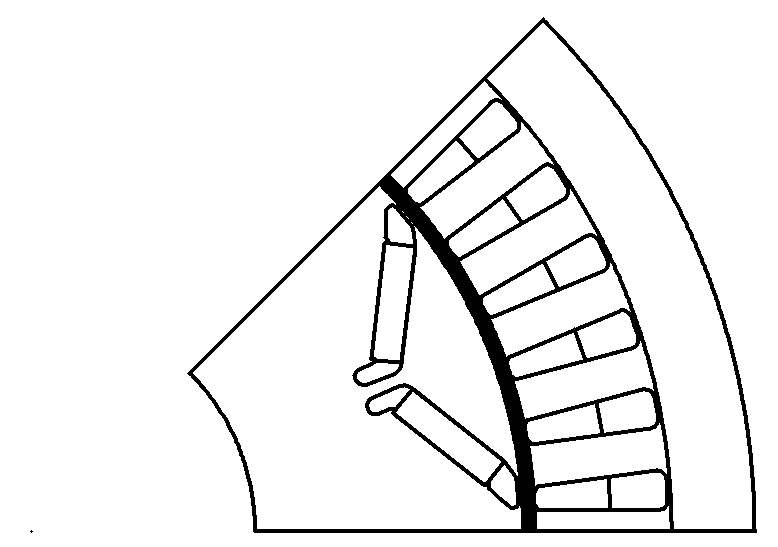
\includegraphics[width=0.47\linewidth]{dxf-orig} \hfill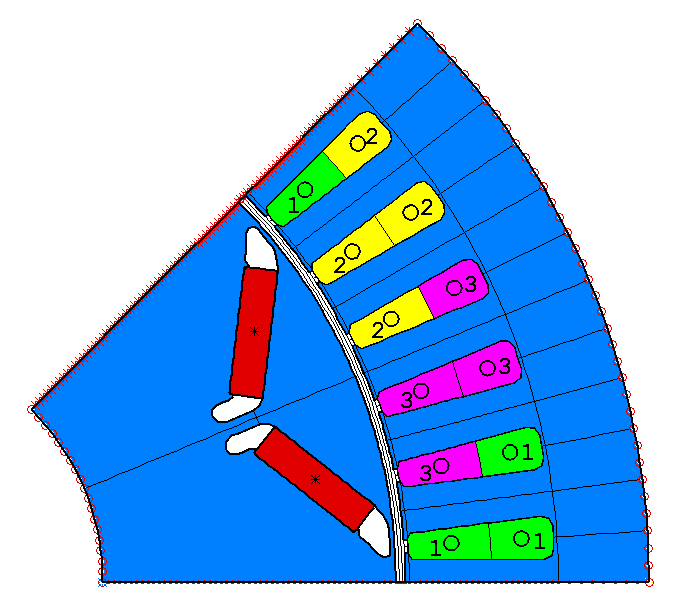
\includegraphics[width=0.4\linewidth]{femag-model}

Dies umfasst folgende Anforderungen:
\begin{enumerate}
\item Identifikation des Luftspaltes und der beiden Maschinenteile, die sich innerhalb und ausserhalb
  der Luftspaltes befinden zusammen mit ihren jeweiligen Innen- und Aussendurchmessern,
\item Identifikation der Symmetrieachsen mit Zerlegung in die kleinstmöglichen Teilbereiche, so dass
  sich mittels Spiegelung und Drehung die vollständige Maschine erstellen lässt,
\item Festlegung der Knotendichte für jeden Teilbereich, so dass möglichst genaue Berechnungsergebnisse
  für das Rastmoment erhalten werden,
\item Identifikation der Subregions Nuten, Stator- und Rotoreisen und Magnet mit Zuordnung der
  jeweiligen Materialeigenschaften,
\item Festlegung der Wicklungen mit Wicklungsschritt, Anzahl Leiter pro Nut, Anzahl Phasen und Anzahl Schichten,
\end{enumerate}
Das Modul ist ausführbar und kann wie folgt aufgerufen werden:
\begin{verbatim}
python -m femagtools.dxfsl.conv [<options>] <DXF filename>
\end{verbatim}
%
\newpage
\enlargethispage{1cm}
\section{Ablauf}
\begin{enumerate}
\item
  Einlesen des DXF-Datei und Erstellung eines NetworkX-Graph-Objektes mit Knoten und Kanten (Nodes, Edges),
\begin{center}  
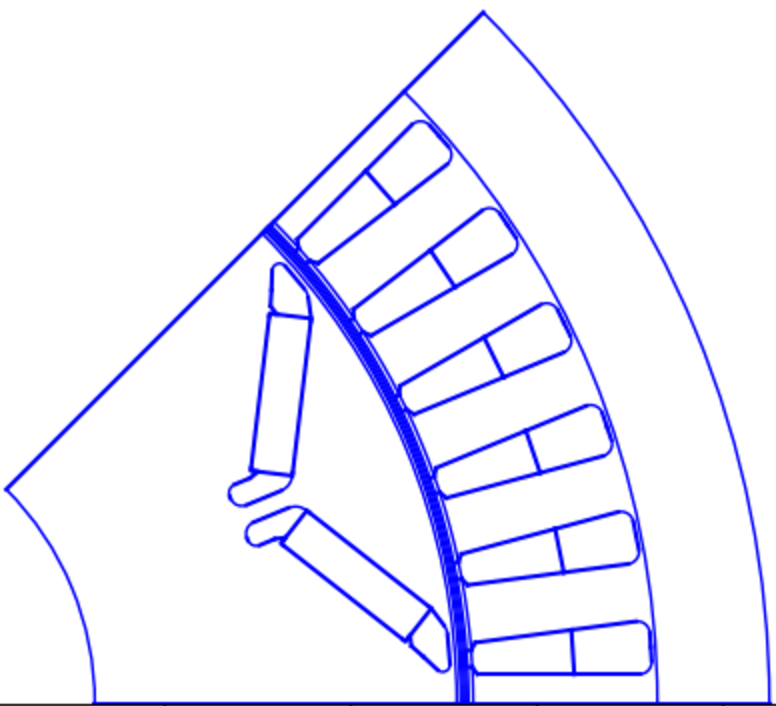
\includegraphics[width=0.45\linewidth]{step1} 
\end{center}
\item Identifikation der Teilbereiche Stator, Rotor und Luftspalt, sowie der Symmetrieachsen und anschliessende
  Zerlegung in je eine Stator- und eine Rotor-Teilnut, % (falls nötig mit Angabe der Luftspaltduchmesser)
  
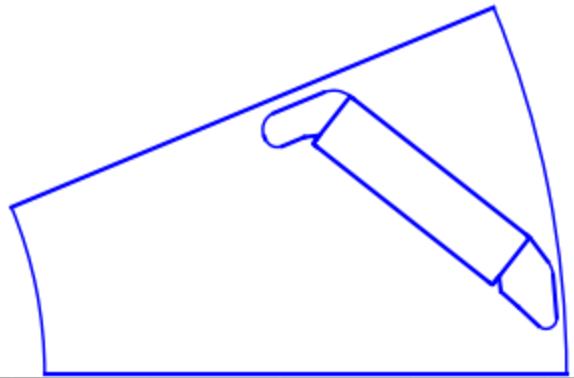
\includegraphics[width=0.45\linewidth]{step2}\hfill 
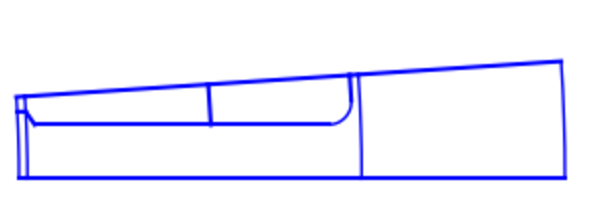
\includegraphics[width=0.45\linewidth]{step4} 
\item
  Hinzufügen von Hilfslinien für die Vernetzung,
\item
  Bestimmung der geschlossenen Bereiche und Ausgabe in FSL-Format, wobei die Knotendichte ausgehend vom
  Luftspalt schrittweise reduziert wird und jeder Bereich mit create\_mesh\_se vernetzt wird. 
\end{enumerate}

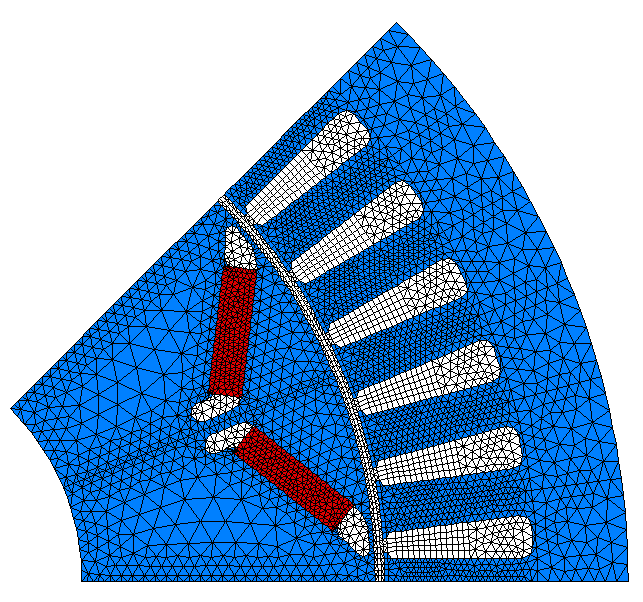
\includegraphics[width=0.45\linewidth]{mesh}\hfill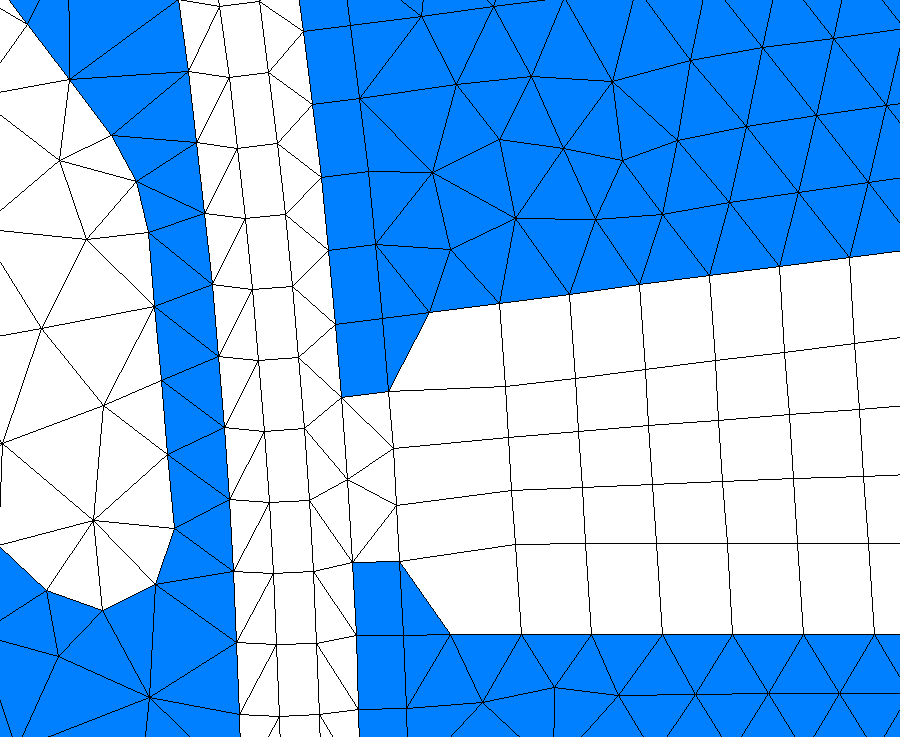
\includegraphics[width=0.45\linewidth]{airgap} 
%
\section{Kommandozeilenparameter}

Folgende Parameter können beim Start gesetzt werden.
\begin{itemize}
\item Filename der einzulesenden DXF-Elemente
\item {\bfseries{\LongArg{fsl}}}\\
      erstellt Dateien mit FSL-Anweisungen (default)
                
\item {\bfseries{\LongArg{split}}}\\
		prüft die eingelesenenen Elemente auf sich schneidende oder berührende Linien.
		In diesen Fällen werden die betroffenen Elemente so aufgeteilt,
		dass an allen Berührungs- und Schnittpunkten auch ein regulärer Knoten vorhanden ist. 
       Diese Option kann notwendig sein, falls keine Symmetrien gefunden werden.
		
\item {\bfseries{\LongArg{view}}}\\
		zeigt die Geometrie in einer Graphik an. Es findet keine weitere Bearbeitung statt.
		
\item {\bfseries{\LongArg{plot}}}\\
		zeigt die Zwischenresultate der verschiedenen Arbeitsschritte als Graphik an.
		
\item {\bfseries{\LongArg{airgap} Radius (float)}}\\
		Wenn mehrere Luftspalt-Kandidaten vorhanden sind, wird die Verarbeitung abgebrochen und
		die Kandidaten werden angezeigt. Mit diesem Parameter wird der innere Radius festgelegt.
		Falls kein Luftspalt vorhanden ist, das Programm aber gleichwohl einen Luftspalt
		identifiziert, kann die Luftspaltidentifikation mit einem negativen Wert unterbunden werden.

\item {\bfseries{\LongArg{airgap2} Radius (float)}}\\
		Wenn im Luftspalt zusätzliche, unnötige Linien vorhanden sind, können diese mit der
		Angabe \Slanted{airgap2} eliminiert werden. Alle Linien zwischen \Slanted{airgap} und
		\Slanted{airgap2} werden damit entfernt.
		
\item {\bfseries{\LongArg{symtol} Toleranzwert (float)}}\\
		Wenn ohne sichtbaren Grund keine Symmetrieachsen gefunden werden, können mit diesem Parameter
		die Toleranzbedingungen beeinflussz werden.
		(siehe auch \Slanted{rtol})
		
\item {\bfseries{\LongArg{rtol} Relativer Toleranzwert (float)}}\\
		Zum ermitteln, ob Knoten als \Slanted{gleich} zu betrachten sind, werden intern relative
		und absolute Abweichungen toleriert. Der Default-Wert ist bei beiden 1e-03. Im Femag
		entspricht dies der Variablen \Slanted{pickdist}.\\
		Die Parameter \Slanted{rtol} und \Slanted{atol} sollten nur bei Maschinen übersteuert 
		werden, die mit dem CAD etwas ungenau konstruiert wurden.
		
\item {\bfseries{\LongArg{atol} Absoluter Toleranzwert (float)}}\\
		(siehe \Slanted{rtol})
		
\item {\bfseries{\LongArg{debug}}}\\
		Durch diese Option werden zusätzliche Informationen (z.B Plots) ausgegeben.
\end{itemize}

\section{Voraussetzungen}
Der Converter sucht geschlossene Regionen und versucht anhand von Regelmässigkeiten die
Symmetrieachsen zu setzen.
\begin{center}
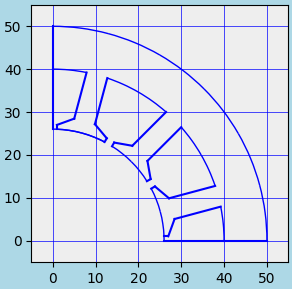
\includegraphics[width=0.45\linewidth]{BspStator}
\end{center}
Bei diesem Beispiel findet der Converter keine Regionen.
Durch zusätzliche Linien können Wicklungsbereiche und damit auch Symmetrieachsen
gefunden werden.

Beispiel: Durch das Einziehen einer Verbindung im Nutschlitz
 wird die Wicklung und der am Luftspalt (airgap) liegende leere Bereich
(Luft) erkannt und der Converter findet eine achsiale Symmetrieachse.
\begin{center}
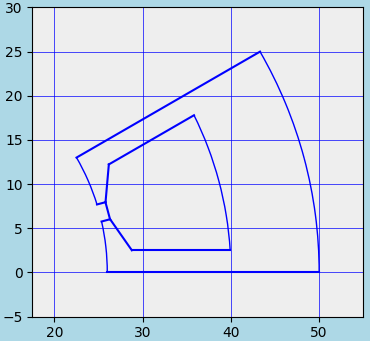
\includegraphics[width=0.45\linewidth]{BspWindings}
\end{center}
Die Wicklungsbereiche werden nicht automatisch durch eine Spiegelung halbiert. Ist das erwünscht,
muss an der entsprechenden Stelle eine Trennlinie erstellt werden.
Dadurch kann auch eine zweilagige Wicklung hineingelegt werden.
\end{document}
